\documentclass{beamer} 	% Full presentation
%\documentclass[trans]{beamer} 			% Transparency mode (no overlays)
%\PassOptionsToPackage{gray}{xcolor}
%\documentclass[handout]{beamer} 	% Handout mode		
 
\ProvidesClass{mbeamer}
\NeedsTeXFormat{LaTeX2e}

\RequirePackage{ifthen}
\RequirePackage{calc}

\AtEndOfClass{\RequirePackage{microtype}}
\DeclareOption*{\PassOptionsToClass{\CurrentOption}{beamer}}
\ProcessOptions*
\LoadClass{beamer}

\RequirePackage[utf8]{inputenc}
\RequirePackage[T1]{fontenc}

\RequirePackage[british]{babel}
\RequirePackage{etex}

% Fonts
\usepackage{mathpazo}
\RequirePackage{libertine}
\renewcommand*\ttdefault{txtt}

%\renewcommand*\sfdefault{\sfdefault}  		% Only if the base font of the document is to be sans serif
%\renewcommand*\ttdefault{lmtt}						% use latin modern typewriter for typewriter fonts (i.e., listings)
%\renewcommand*\sfdefault{lmss}						% use latin modern sans serif for main text
%\RequirePackage[adobe-utopia]{mathdesign}  		% use Adobe Utopia for serif text (i.e., mainly titles) and Mathdesign for math fonts
%\RequirePackage{fourier}
%\RequirePackage{DejaVuSansCondensed}
%\RequirePackage[scaled=.77]{beramono}

% Font features
\RequirePackage{lettrine}
\RequirePackage{accents}
\RequirePackage{xspace}

% Math
\RequirePackage{amsmath}
\RequirePackage{mathtools}
\RequirePackage{nicefrac}

\renewcommand*{\dot}[1]{\skew{2}{\accentset{\mbox{\bfseries .}}}{{#1}}}
\newcommand*{\Chat}{\skew{3}{\hat}{c}}
\newtheorem{prop}{Proposition}

% Graphics
\RequirePackage{fancybox,graphicx}
\RequirePackage{pgfpages}
\RequirePackage{animate}
\RequirePackage{pgfplots}
\usetikzlibrary{intersections}
\pgfplotsset{compat=newest}
	
% Sweave
\RequirePackage{sweave}

% Tables
\RequirePackage{booktabs}

% Miscellaneous
\RequirePackage[os=win]{menukeys}

% Custom functions
\colorlet{Bgreen}{green!50!black} 
\definecolor{Bblue}{rgb}{0.23,0.4,0.7}

\newenvironment{proenv}{\only{\setbeamercolor{local structure}{fg=Bgreen}}}{}
\newenvironment{conenv}{\only{\setbeamercolor{local structure}{fg=Red}}}{}

\newcommand*\proitem{%
  \item[\color{Bgreen}\scalebox{0.8}{$\blacktriangleright$}]}
\newcommand*\conitem{%
  \item[\color{Red}\scalebox{0.8}{$\blacktriangleright$}]}

\newcommand{\Rv}[1]{\texttt{\textcolor{OliveGreen}{{#1}}}}
\newcommand{\Rf}[1]{\texttt{\textcolor{BrickRed}{{#1}}}}
\newcommand{\Rt}[1]{\texttt{\textcolor{RoyalPurple}{{#1}}}}
\newcommand{\Rs}[1]{\texttt{\upshape \textcolor{Black}{{#1}}}}
\newcommand{\R}{\texttt{R}\xspace}

\definecolor{higlblue}{rgb}{0.23,0.40,0.70}% use structure theme to change
\newcommand{\highld}[1]{\textcolor<2>{higlblue}{#1}}
\newcommand{\highl}[1]{\textcolor{higlblue}{#1}}

\newenvironment{myquote}{\list{}{\leftmargin=0pt\rightmargin=10pt}\itshape\item[]}{\endlist}

%%%%%%%%%%%%%%%%%%%%%%%%%%%%%%
% Beamer settings

\setbeamertemplate{navigation symbols}{}

% define \hfilll command to replace \hfill in title alignment
\newcommand{\hfilll}{\hspace{0pt plus 1 filll}}

%% Glossy pretty look for the presentation and transparency (w/o overlays and animations) versions!
\mode<beamer|trans>{
\useoutertheme[glossy]{wuerzburg} %nofootline
\useinnertheme[shadow,realshadow]{chamfered}
\usecolortheme{shark}
}

\setbeamertemplate{frametitle continuation}[from second][(cont'd)]
\usefonttheme{serif} % [stillsansseriftext,stillsansserifsmall]

%% Save up on ink for the 4-up handouts
\mode<handout>{
\setbeamertemplate{footline}[frame number]
\setbeamercolor{background canvas}{bg=white}
\usecolortheme[named=black]{structure} 
%\useoutertheme[nofootline]{wuerzburg}
%\useinnertheme[outline]{chamfered}

\pgfpagesuselayout{4 on 1}[a4paper, border shrink=10mm, landscape]
\pgfpagesuselayout{4 on 1}[a4paper,border shrink=3mm,landscape]
%\pgfpagesuselayout{resize to}[a4paper, landscape, border shrink=3mm]
}


\author{Matteo Sostero}
\title{Title}
\subtitle{Subtitle}

\begin{document}

\begin{frame}
\includegraphics[scale=0.8]{SA_economics_logo_eng.pdf}
\maketitle
\end{frame}

\begin{frame}
\frametitle{Outline}
\tableofcontents
\end{frame}

\section{Blocks and lists}
\begin{frame}
    \frametitle{Some lists and warnings}
    \begin{itemize}[<+->]
	\item First item
	\item Second item
	\item \alert{Important Warning!}	
	\item Hyperlink 	\highl{\hyperlink{Hayek-quote}{Hayek (1945)}} \only<4>{\hypertarget{Hayek-back}{}}
	\end{itemize}
	\pause[\thebeamerpauses]
	\begin{alertblock}{Even more important warning!}
	This is an important warning.
	\end{alertblock}
\end{frame}


\begin{frame}
\frametitle{Why \LaTeX?}
\framesubtitle{From \url{http://www.ctan.org/what_is_tex.html}}
\begin{columns}[T]
\begin{column}{.46\textwidth}
\begin{block}{Output Quality}
\begin{itemize}
\item It has the best output.
\item It knows typesetting.
\end{itemize}
\end{block}
\uncover<3->{
\begin{block}{Superior Engineering}
\begin{itemize}
\item It's fast.
\item It's stable.
\item It's not rigid (extensible).
\item Plain text input.
\item Many output types.
\end{itemize}
\end{block}
}
\end{column}
 
\begin{column}{.46\textwidth}
\uncover<2->{
\begin{block}{Freedom}
\begin{itemize}
\item It's free.
\item It runs anywhere.
\end{itemize}
\end{block}
}
\uncover<4->{
\begin{block}{Popularity}
\begin{itemize}
\item It's the standard (in academia and science).
\end{itemize}
\end{block}
}
\end{column}
\end{columns}
\end{frame}

\begin{frame}
    \frametitle{Example blocks} 
 \begin{columns}[T]

\begin{column}{0.45\textwidth}
\begin{exampleblock}{Transparent uncover}
\setbeamercovered{transparent}
\begin{itemize}[<+->]
\item Item 1
\item Item 2
\item Item 3
\end{itemize}
\end{exampleblock}
\end{column}


\begin{column}{0.45\textwidth}
\begin{exampleblock}{Highlighting}
\begin{enumerate}[<alert@+>]
\setbeamercolor{alerted text}{fg=green!50!black} 
\item Item 1
\item Item 2
\item Item 3
\end{enumerate}
\end{exampleblock}
\end{column}
\end{columns}
\end{frame}
% ---

% -----
\section{Code listings}
\begin{frame}[fragile]
    \frametitle{Example of \R code}
    Some code
\begin{Sinput}
binary <- function(i){
    a <- 2^(0:9)
    b <- c(NULL,NA,1,2,3)
    sapply(i,function(x) sum(10^(0:9)[(x %% b)>=a]))
    # Comment
    print("a quote")
}
\end{Sinput}

Some output of another \R command: \Rf{print}\Rs{(...)}\\
\begin{Soutput}
 [1]  1  2  3  4  5  6  7  8  9 10
\end{Soutput}

% See http://texblog.org/2013/03/14/menukeys-typesetting-menu-sequences-directory-path-names-and-keyboard-shortcuts-in-latex/
For saving a file to the desktop, go to \menu[,]{File, Save As...} and navigate to \directory{Users/Username/Desktop}.\\
Alternatively, use the following keyboard shortcuts: \keys{\ctrl+\shift+S} and \keys{\ctrl+\return+\tab}.

\end{frame}
% -----



% --- Formulas
\section{Formulas}
\begin{frame}
    \frametitle{Some impressive-looking formulas \ldots}
    \begin{itemize}[<+->]
	\item Meaningless expression:
	\[ 
	\frac{\partial \mathcal{L} \left(R(t), \phi\right)}{\partial t} \sim  
	\left \lbrace \int_{-\infty}^{+\infty} \frac{\widetilde{\mathcal{H}}(\gamma) \cdot \sqrt{\lim_{t\rightarrow\infty}\exp^{t-1}}}{\sum_{i=1}^\infty \mathbb{E}\left( \dot{x}_i^2\right)} dt \right \rbrace^{-1}
	\]	
	\item Matrices and greek letters
	\[
	\forall \Gamma \Delta\exists \Theta \otimes  \mathbb{R} \succeq
	\begin{bmatrix}
	\alpha & \beta 	  & \gamma &\delta 	&\varepsilon &\zeta  &\eta\\
	\theta & \iota 	 &\kappa & \lambda & \mu 				& \xi		&\pi	\\ 		
	\rho	& \sigma & \tau 		& \phi 			& \chi 	& \psi 				& \omega\\
	\end{bmatrix}
	=
	\begin{bmatrix}
	a_{\ell \kappa} & \ldots& \tau_{\ell i}\\
	\vdots & \ddots & \vdots \\
	\tau_{yj} & \ldots & a_{nn}\\
	\end{bmatrix}
	\]
	
	\[\dot{a}\; \dot{x}\; \dot{y}\; \dot{w}\; \dot{z} \;\dot{\tau}\]
	\end{itemize}
\end{frame}
% -----

\section{Plots}
% -----
\begin{frame}[fragile]
\frametitle{A plot}
	\begin{center}
		\begin{tikzpicture} 
		\begin{axis}[
		axis x line=middle, 
		axis y line=left,
		domain=0:2,
		legend pos= north west,
		xlabel=$x$,
		ylabel=$ f(x)$,
		ytick={0,1,2,3},
		every axis y label/.style={at={(current axis.above origin)},anchor=north east}
		]
		\addplot[blue,mark=none,domain=0:2.01,samples=101] {(x^2)}; 
		\addlegendentry{$x^2$}
		\only<2>{
		\addplot[red,mark=none,domain=0:2,samples=101] {sqrt(x)}; 		
		%\addplot[red,mark=none] gnuplot[domain=0:2,samples=101] {sqrt(x)}; 		
		\addlegendentry{$\sqrt{x}$}
		}
		\end{axis}
		\end{tikzpicture}
	\end{center}
\end{frame}


\begin{frame}[fragile]
\frametitle{A plot}
	\begin{center}
		\begin{tikzpicture}
\begin{axis}[
  height=5cm, width=10cm,
  xmin=-3.5, xmax=3.5,
  ymin=0, ymax=0.50,
  ytick={0},
  axis x line=bottom, axis y line=center,
  xlabel=$x$, ylabel=$f(x)$,
  every axis x label/.style={at={(current axis.right of origin)},anchor=north west},
  every axis y label/.style={at={(current axis.above origin)},anchor=north west}
]

% Draw normal curve
\addplot[Cblue,thick,smooth,domain=-3.5:3.5] {
  (1/(sqrt(2*pi)))*exp(-(x^2)/2) 
};

% Draw vertical line:
\only<2->{
  \draw [BrickRed,thick] (axis cs:-1.5,0) -- (axis cs:-1.5,0.1295176);
}

% Draw area
\only<3->{
  \addplot[fill=Cblue,opacity=0.4,smooth,domain=-3.225:-1.51] { (1/(sqrt(2*pi)))*exp(-(x^2)/2) } \closedcycle;
}
\end{axis}
\end{tikzpicture}

	\end{center}
\end{frame}
% -----


% --- Tabulars
\section{Tabulars}
\begin{frame}
    \frametitle{Tables}
    \begin{center}
		\begin{tabular}{ccc}
		\toprule
  	    	Title left & & Title right  \\
		 	\midrule  \pause
  	        Left 1 & Center 1 & Right 1  \\ 
			Left 2 & Center 2 & Right 2   \\
			\bottomrule
		\end{tabular}
	\end{center}
\end{frame}


\section{References}
\begin{frame}
\frametitle{References}
\begin{thebibliography}{9}
\setbeamertemplate{bibliography item}[book]
\bibitem{1} Nelson, R. R., and Winter, S. G. 1982. \emph{An Evolutionary Theory of Economic Change.} Cambridge, Massachusetts: Belknap press.
\setbeamertemplate{bibliography item}[article]
\bibitem{2} Friedman, M. 1953. ``The Methodology of Positive Economics.''  In \emph{Essays in
Positive Economics.} Chicago : University of Chicago Press.
\bibitem{3} Alchian, A . A . 1950. ``Uncertainty, Evolution and Economic Theory.'' \emph{Journal
of Political Economy} 58 : 211 - 222.
\setbeamertemplate{bibliography item}[book]
\bibitem{4} Koopmans, T. C. 1 957. \emph{Three Essays on the State of Economic Science.} New
York: McGraw-Hill.
\end{thebibliography}
\end{frame}

\appendix

\begin{frame}[label=Hayek-quote]
\frametitle{Hayek's problem\hfilll \hyperlink{Hayek-back}{\beamerreturnbutton{Literature}}}
\begin{block}{}
\begin{columns}
\begin{column}{0.25\textwidth}
	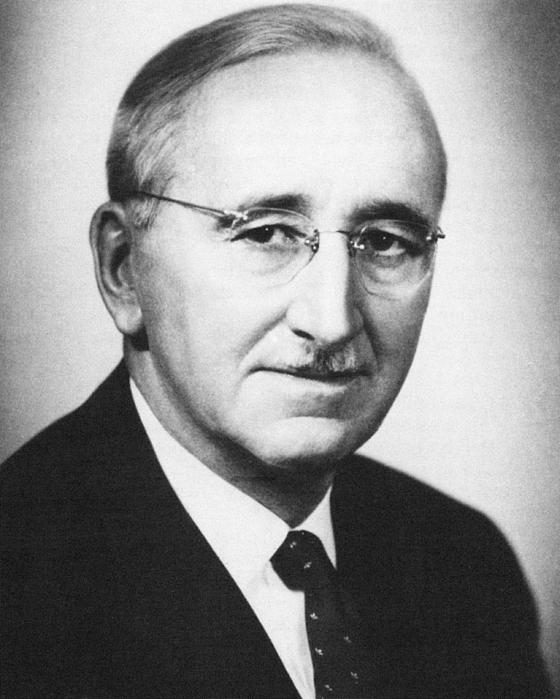
\includegraphics[width=\textwidth]{Hayek.jpg}
\end{column}
\begin{column}{0.7\textwidth}
\begin{myquote}
	\lettrine[findent=3.5pt,nindent=-3pt]{T}{he} peculiar character of the problem of a rational economic order
	is determined precisely by the fact that the \highld{knowledge of the circumstances
	of which we must make use never exists in concentrated or
	integrated form}, but solely as the dispersed bits of incomplete and
	frequently contradictory knowledge which all the separate individuals
	possess. 
\end{myquote}
\end{column}
\end{columns}
\flushright Hayek (1945), 	\emph{The use of Knowledge in Society}\only<2>{, \highld{emphasis added}}
\end{block}	
\end{frame}

%\begin{frame}<presentation>
%\frametitle{Animation}
%\centering 
%\animategraphics[controls,buttonsize=0.3cm,width=0.8\paperwidth,poster=last]{6}{"./Frames/ergo"}{1}{100}
%\end{frame}

\end{document}
